% Public AI Switzerland — Website User Guide
% Build with Tectonic (bundles its own TeX engine, no system TeX needed):
%   tectonic docs/user-guide/main.tex
% Public Sans is embedded via fontspec from the system font files.
\documentclass[11pt]{book}
\usepackage[a4paper,margin=2.2cm]{geometry}
\usepackage{fontspec}
\setmainfont{PublicSans}[
  Path=/Users/joshuavargas/Library/Fonts/,
  Extension=.ttf,
  UprightFont=PublicSans-VariableFont_wght,
  ItalicFont=PublicSans-Italic-VariableFont_wght,
  BoldFont=PublicSans-VariableFont_wght,
]
\usepackage{graphicx}
\usepackage{xcolor}
\usepackage{hyperref}
\usepackage{listings}
\usepackage{fancyhdr}
\usepackage{titlesec}
\usepackage{enumitem}

\definecolor{brandred}{HTML}{C82632}
\definecolor{ink}{HTML}{17212C}
\definecolor{muted}{HTML}{596571}
\definecolor{codebg}{HTML}{F1F3F5}

\hypersetup{colorlinks=true, linkcolor=brandred, urlcolor=brandred}
\lstset{basicstyle=\ttfamily\small, backgroundcolor=\color{codebg}, frame=single, rulecolor=\color{muted}, breaklines=true, columns=fullflexible}
\titleformat{\chapter}{\normalfont\Huge\bfseries\color{brandred}}{}{0pt}{}
\titleformat{\section}{\normalfont\Large\bfseries\color{ink}}{}{0pt}{}
\pagestyle{fancy}
\fancyhf{}
\fancyhead[L]{\small\color{muted}Public AI Switzerland --- Website User Guide}
\fancyhead[R]{\small\color{muted}\thepage}
\renewcommand{\headrulewidth}{0.4pt}

\title{Website User Guide\\[4pt]\large A friendly handbook for contributing content to publicai.ch}
\author{Public AI Switzerland}
\date{2 November 2026}

\begin{document}
\maketitle
\tableofcontents

\chapter{Welcome}
This handbook shows you how to update the Public AI Switzerland website: editing pages, publishing news, and changing the navigation. You do not need to know React or any programming language --- everyday content work happens in plain text files and one configuration file.

The website speaks five languages: English (at the root address), German, French, Italian, and Romansh. Each page keeps all of its translations in a single file, so you can always see which languages are still missing.

\begin{figure}[h]
\centering
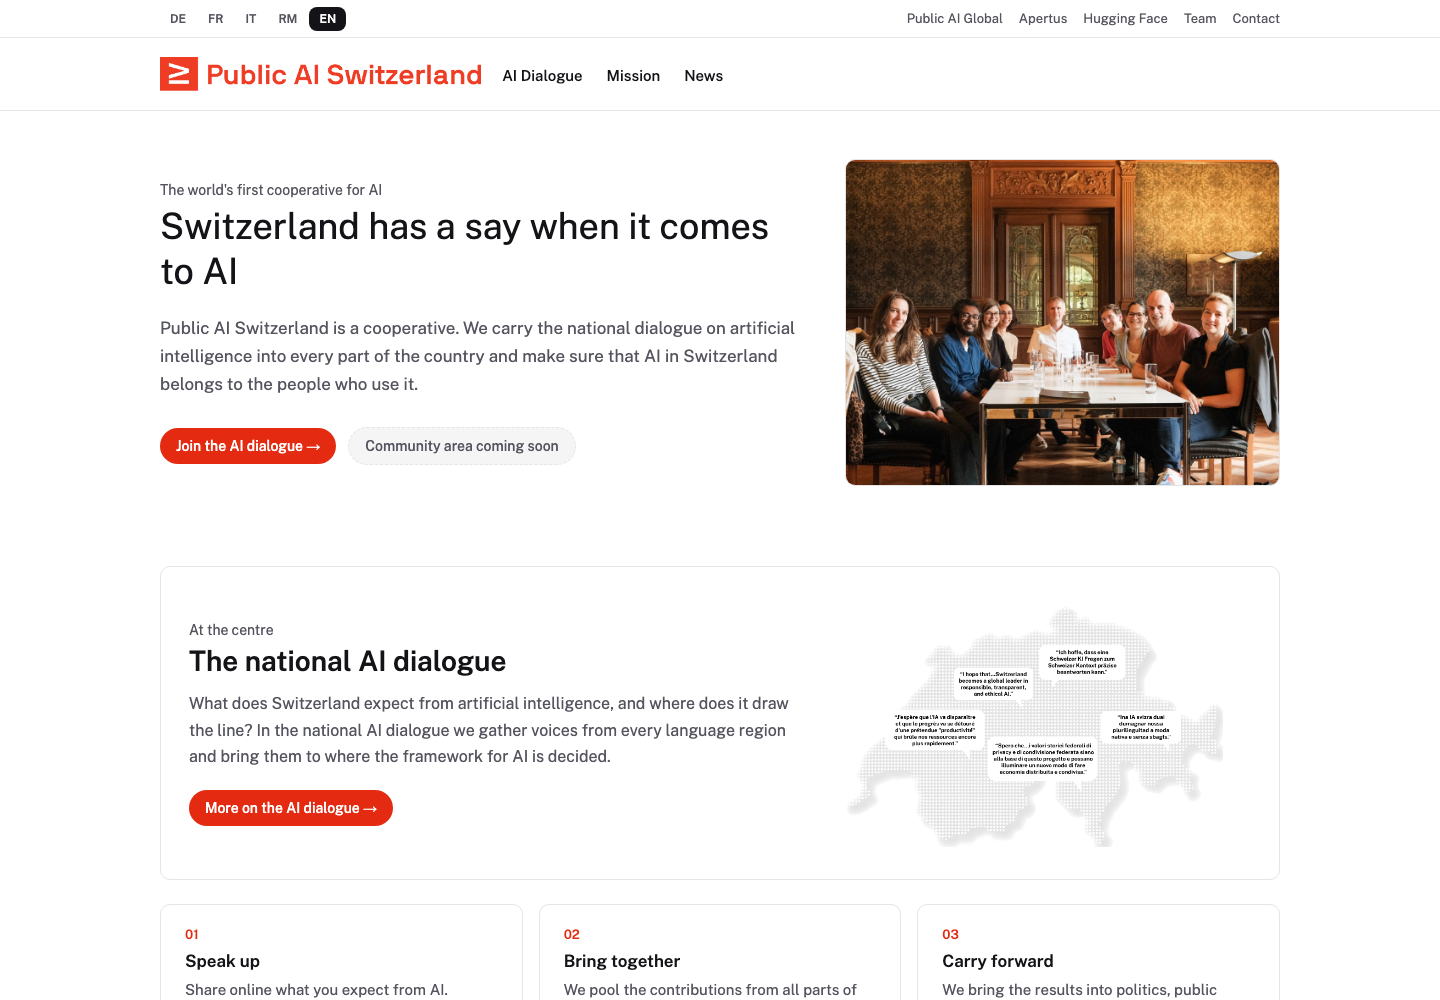
\includegraphics[width=0.9\textwidth]{screenshots/home.png}
\caption{The English home page in a local preview.}
\end{figure}

\chapter{The big picture}
Three places cover almost all everyday work:
\begin{itemize}
  \item \texttt{content/} --- the text of every page, in MDX files (Markdown plus optional layout blocks).
  \item \texttt{public/assets/} --- images and downloadable files.
  \item \texttt{config.json} --- the header menus, footer links, news categories, redirects, and a few switches.
\end{itemize}

Everything else is generated. The build turns your MDX files into static pages, rebuilds the sitemap, checks every internal link, and refuses to publish a page that nothing links to.

To find the file behind an address, drop the slashes: \texttt{/mission/} comes from \texttt{content/cooperative/mission.mdx}, and the German page is \texttt{/de/mission/}. News addresses include the date: \texttt{/news/2026-09-24-zurich-hackathon/}.

\chapter{Run a local preview}
A preview on your own machine lets you check changes before anyone else sees them.

\begin{lstlisting}[language=bash]
git clone https://github.com/forpublicai/publicai.ch.git
cd publicai.ch
corepack enable
yarn install --immutable
yarn dev
\end{lstlisting}

Open the printed address, usually \texttt{http://localhost:5173/}. Save an edit and look at the browser. Stop the server with Ctrl+C.

\textbf{Restart \texttt{yarn dev}} whenever you add or delete a file, add or remove a language section, or change a page's \texttt{draft} status. Plain wording edits refresh on their own.

\chapter{Edit an existing page}
\begin{enumerate}[label=\arabic*.]
  \item Find the file whose name matches the address --- for \texttt{/mission/} that is \texttt{content/cooperative/mission.mdx}.
  \item Find the language section you want, for example \texttt{<!-- locale: en -->}.
  \item Edit the text below that marker, stopping at the next marker.
  \item If the heading or summary changed, update that language's \texttt{title} and \texttt{description} in the frontmatter at the top.
  \item Save, check the preview, and run \texttt{yarn build} before handing over the change.
\end{enumerate}

\begin{figure}[h]
\centering
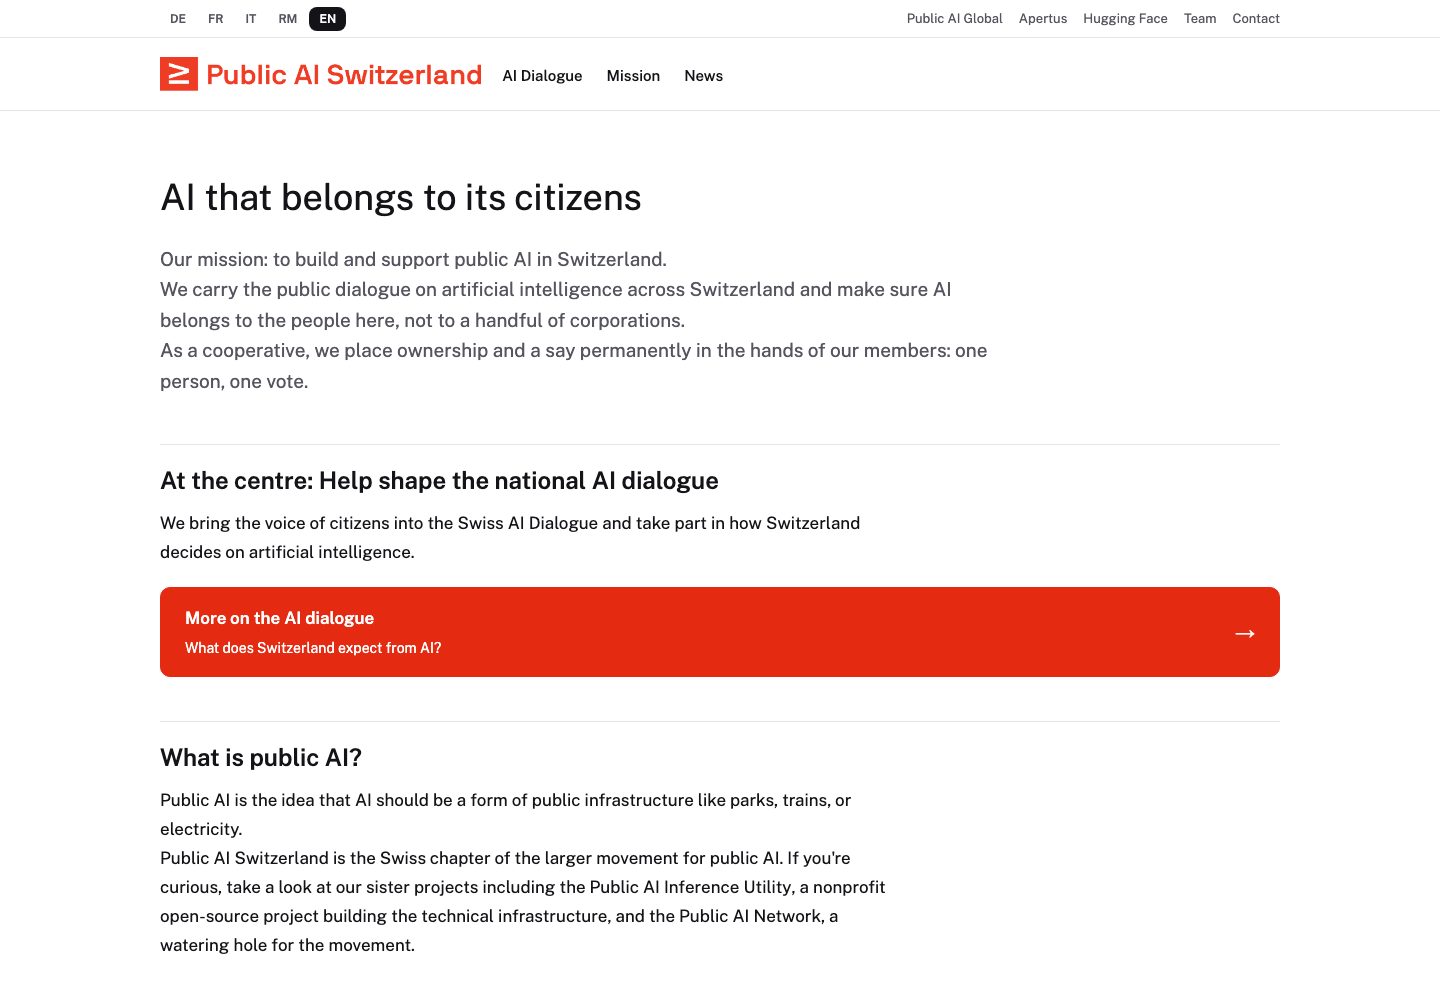
\includegraphics[width=0.9\textwidth]{screenshots/mission.png}
\caption{The Mission page, rendered from its MDX file.}
\end{figure}

An MDX file has two parts: the frontmatter between the \texttt{---} lines (title, description, flags), and the body divided by language markers. Keep both in place.

\chapter{Create a new page}
Copy the template and give the copy a unique, stable filename (lowercase letters, numbers, hyphens; avoid the reserved names \texttt{news} and \texttt{authors}):

\begin{lstlisting}[language=bash]
cp content/templates/page-template.mdx content/community/workshops.mdx
\end{lstlisting}

Delete the template's instruction paragraph before the first language marker --- no body text may sit above a marker. Then write your content under the markers, one per language.

A minimal English-only page looks like this:

\begin{lstlisting}
---
title: Workshops
description: Meet the community and take part in our public AI workshops.
---

<!-- locale: en -->

Come and learn with us.

## What to expect

[Read our mission](/mission)
\end{lstlisting}

This creates \texttt{/workshops/} in English only. Add German, French, Italian, and Romansh sections to create \texttt{/de/workshops/} and so on.

\textbf{Link the new page} from an existing page or from \texttt{config.json}, otherwise the build's reachability check fails. While drafting, set \texttt{draft: true}; drafts have no routes at all, even locally.

\chapter{Work in five languages}
The language codes are \texttt{en}, \texttt{de}, \texttt{fr}, \texttt{it}, and \texttt{rm}. Each marker goes on its own line, each language appears at most once, and at least one section is required.

Translations are written by the author, not generated automatically. That is deliberate: legal text such as the statutes must not be machine-translated, and every translation should be reviewed by a person. When a fact, date, or link changes, review the other language sections too.

Translate the metadata as well:
\begin{lstlisting}
title: Workshops
title_fr: Ateliers
description: Discover our workshops and join the next gathering.
description_de: Entdecken Sie unsere Workshops und das naechste Treffen.
\end{lstlisting}
A missing \texttt{title\_xx} falls back to English, then German, then the base field --- so set explicit overrides for each finished translation.

Only languages with a section get a page route. Requesting a missing translation can produce a 404 rather than a fallback, so click through every language when reviewing. The build writes \texttt{untranslated-sections-report.txt} listing any gaps.

\chapter{Format text and add images}
Ordinary Markdown works everywhere: headings with \texttt{\#\#}, bold, lists, and links. Internal links such as \texttt{/mission} automatically carry the current language prefix.

Save images under \texttt{public/assets/} and reference them from \texttt{/assets/}:
\begin{lstlisting}
<Figure
  src="/assets/images/workshops/workshop.jpg"
  alt="Participants discussing ideas around a workshop table"
  caption="A community workshop in Zurich."
/>
\end{lstlisting}
Write alt text that conveys the useful information, and translate captions and alt text per language.

Ready-made blocks cover common layouts:
\begin{lstlisting}
<Lead>A short introduction that stands out.</Lead>
<Callout variant="info">Registration details will be shared soon.</Callout>
<CTA title="Read our mission" to="mission" />
\end{lstlisting}
\texttt{to="..."} takes a page slug; external buttons use \texttt{href="https://..."}. The full catalogue --- stat grids, accordions, team cards, poster downloads, video embeds --- is in \texttt{docs/reference/components.md}. Embeds only accept hosts listed in \texttt{embeds.allowlist} in \texttt{config.json}.

\chapter{Publish a news article}
A news article is an MDX file whose frontmatter has both \texttt{date} and \texttt{category}.

\begin{lstlisting}[language=bash]
cp content/templates/news-template.mdx content/news/2026-11-09-community-workshop.mdx
\end{lstlisting}

Use the publication date at the start of the filename and in the frontmatter. The category must be one of \texttt{news.categories} in \texttt{config.json}: \texttt{Dialog}, \texttt{Genossenschaft}, \texttt{Community}, \texttt{Medien}, \texttt{Technik}.

\begin{lstlisting}
---
title: A community workshop
description: Our community explored public AI and planned the next steps.
date: 2026-11-09
category: Community
---

<!-- locale: en -->

We met to exchange ideas and learn together.
\end{lstlisting}

The article then appears automatically at \texttt{/news/2026-11-09-community-workshop/}, in the News listing (newest first), and in the home teaser (latest three). Set \texttt{draft: true} to hide it while working, and use \texttt{externalUrl} when the article really lives on another site.

\begin{figure}[h]
\centering
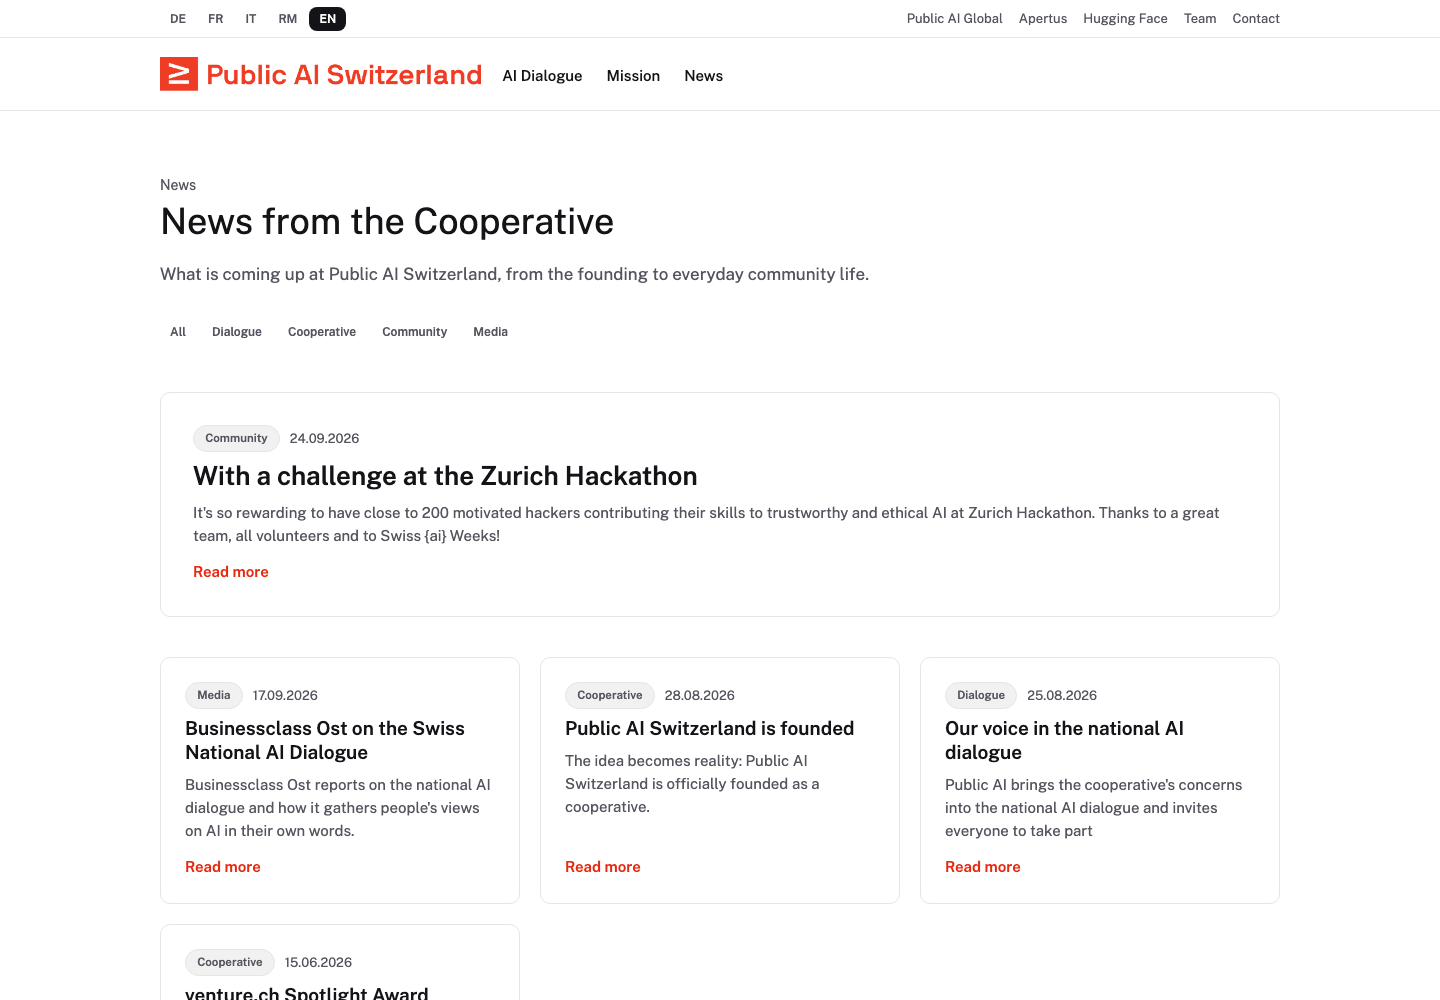
\includegraphics[width=0.85\textwidth]{screenshots/news.png}
\caption{The generated News listing.}
\end{figure}

\chapter{Menus and footer}
All navigation lives in \texttt{config.json}. Each menu item needs a five-language \texttt{label} and exactly one target:
\begin{itemize}
  \item \texttt{"page": "mission"} --- an internal page slug;
  \item \texttt{"url": "https://publicai.co"} --- an external or \texttt{mailto:} link;
  \item \texttt{"children": [...]} --- a one-level dropdown of further items.
\end{itemize}

\begin{lstlisting}
{
  "label": { "en": "Workshops", "de": "Workshops", "fr": "Ateliers",
             "it": "Workshop", "rm": "Lavuratoris" },
  "page": "workshops"
}
\end{lstlisting}

Keep JSON punctuation intact (double quotes, commas between entries, none after the last). The build fails with the exact config path if a label is missing a language or a \texttt{page} slug does not exist. The footer works the same way, including a compact newsletter sign-up form below the tagline; check narrow screens too, since both menus fold into one mobile menu.

\chapter{Next steps}
Before handing over a change, run the full check chain:
\begin{lstlisting}[language=bash]
yarn lint
yarn typecheck
yarn test
yarn build
yarn test:e2e   # needs Chromium: yarn playwright install chromium
\end{lstlisting}

Then open a preview of the built site with \texttt{yarn build \&\& yarn preview} (usually \texttt{http://localhost:4173/}). The live website only changes when a new build is deployed, and only \texttt{build/client/} is ever uploaded --- never commit generated output.

For details, see the how-to guides and references in \texttt{docs/}, the illustrated \texttt{docs/pdf/quick-guide-for-content-contributors.pdf}, and \texttt{docs/deploy/server-admin-guide.md} for deployment.

\end{document}
